\newthought{\textbf{Nurani Harum Fardaniah - 2020903430034 - TRKJ 3B}}

\newday{\textbf{1 Desember 2022}}
\begin{enumerate}
\item Kendala dan Solusi
\newline Kendala :\\
Saat melakukan penginstalan hadoop tidak ada kendala apapun. Namun pada saat melakukan konfigurasi hadoop terdapat kendala pada saat melakukan hdfs namenode -format. Perintah ini tidak mau dijalankan karena ada kesalahan dalam penulisan pada file core-site.xml
Saat melakukan perintah jps pun hanya menampilkan 1 saja.

Solusi :\\
Melakukan perubahan penulisan pada file core-site.xml, setelah itu perintah hdfs namenode -format dapat dijalankan dan saat melakukan perintah jps akhirnya muncul ada 5.

\item Kesimpulan
\newline Praktikum penginstalan hadoop dan konfigurasi hadoop berhasil dijalankan sesuai perintah-perintah yang ada.

\begin{figure}[!ht]
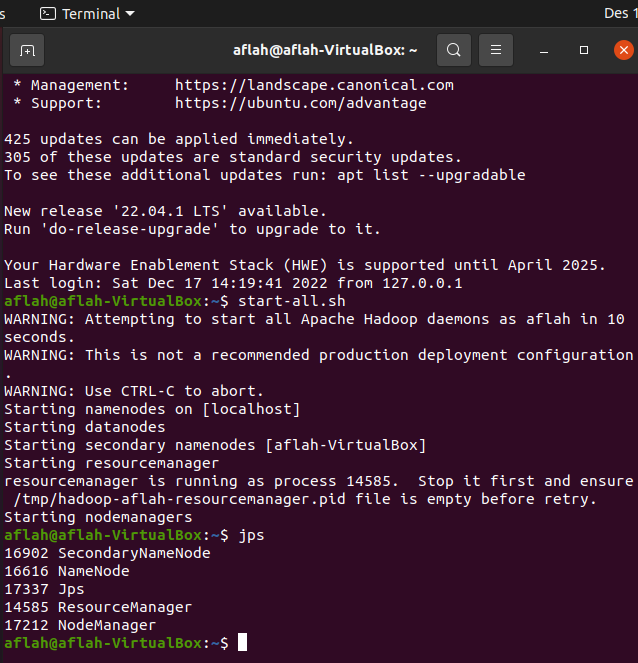
\includegraphics[width=\textwidth]{jps}
\caption{hasil dari jps}
\label{gam:perkuliahan-25-11}
\end{figure}

\begin{figure}[!ht]
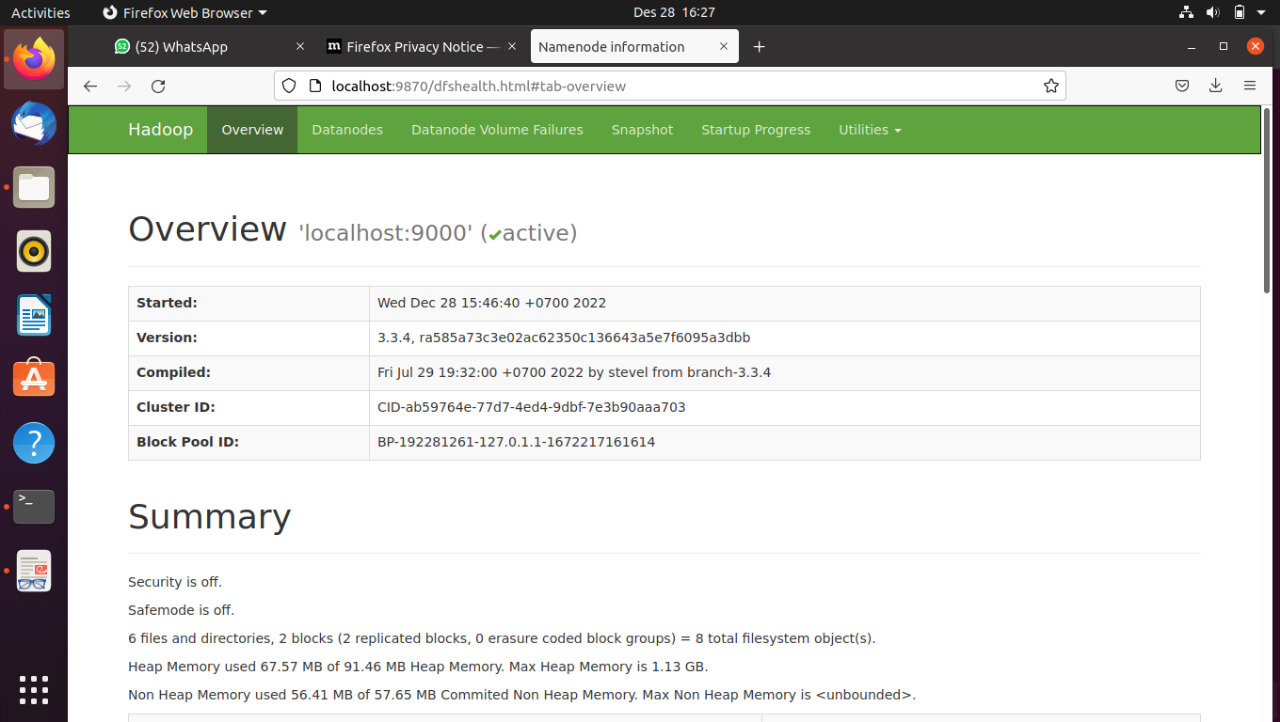
\includegraphics[width=\textwidth]{localhost9870}
\caption{hasil dari localhost 9870}
\label{gam:perkuliahan-25-11}
\end{figure}

\newpage
\begin{figure}[!ht]
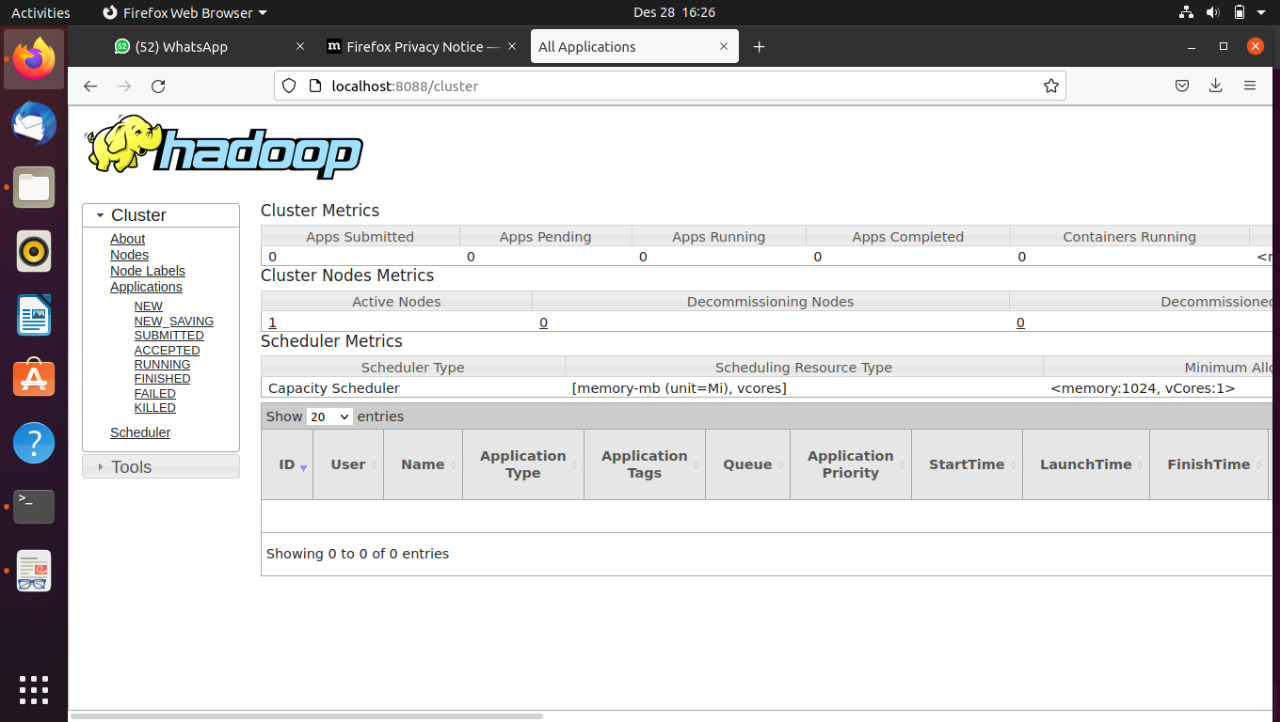
\includegraphics[width=\textwidth]{localhost8088}
\caption{hasil dari localhost 8088}
\label{gam:perkuliahan-25-11}
\end{figure}

\end{enumerate}

\newday{\textbf{2 Desember 2022}}
\begin{enumerate}
\item Kendala dan Solusi
\newline Tidak ada kendala apapun saat melakukan program WordCount bawaan Hadoop

\item Kesimpulan
\newline Praktikum berhasil dilakukan sesuai dengan perintah-perintah yang ada. WordCount sendiri merupakan program untuk menghitung jumlah kata yang ada pada data.


\begin{figure}[!ht]
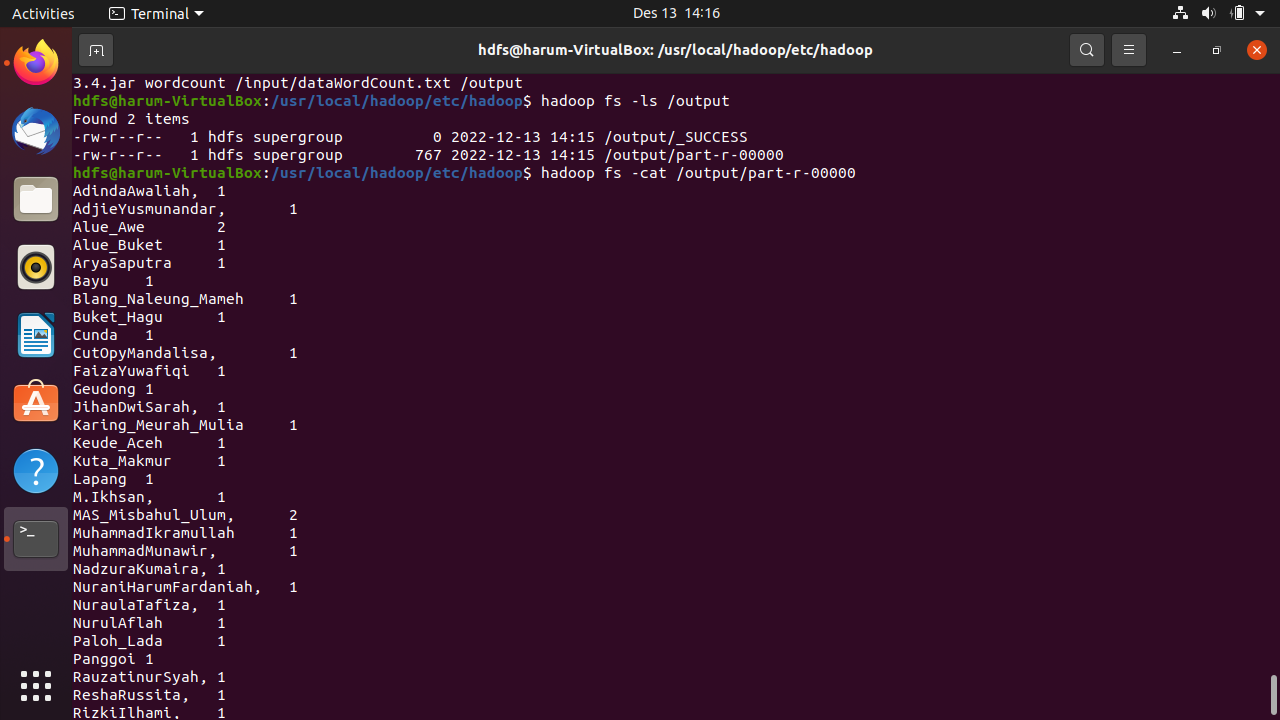
\includegraphics[width=\textwidth]{6-7a}
\caption{Hasil dari langkah 6 dan 7}
\label{gam:perkuliahan-25-11}
\end{figure}
\newpage
\begin{figure}[!ht]
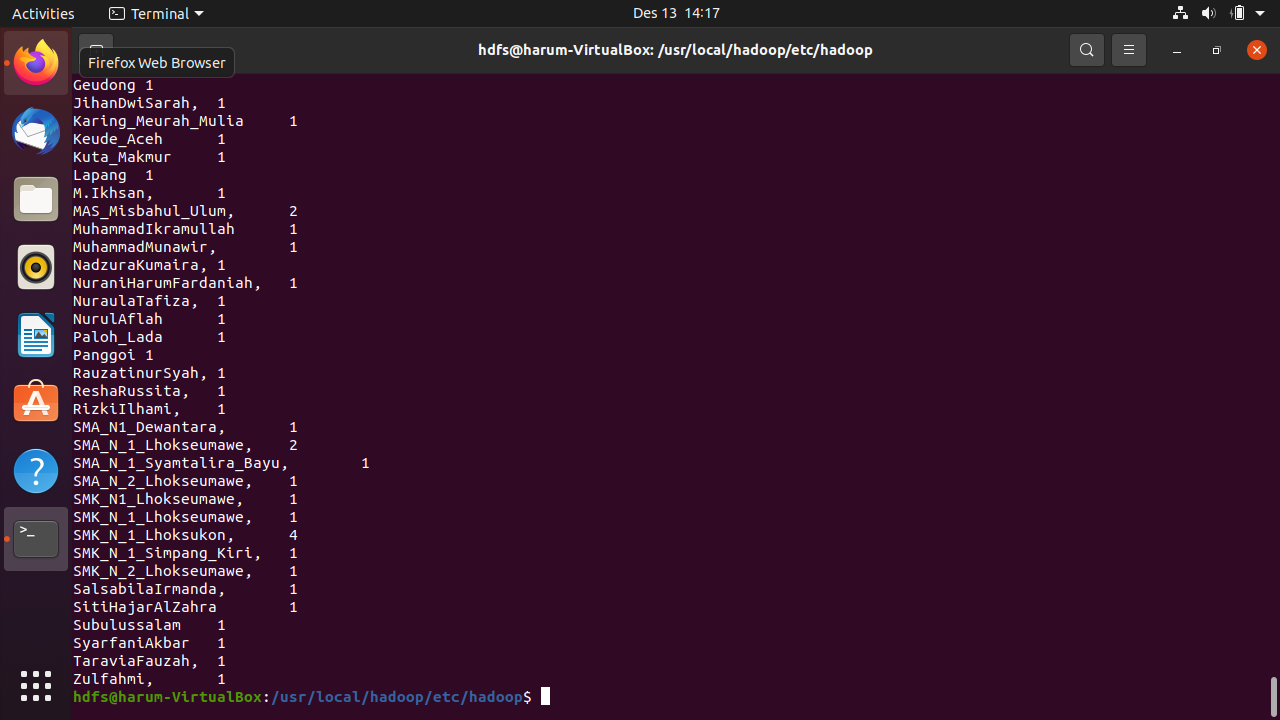
\includegraphics[width=\textwidth]{7b}
\caption{Hasil dari langkah 7}
\label{gam:perkuliahan-25-11}
\end{figure}

\end{enumerate}

\newday{\textbf{8 Desember 2022}}
\begin{enumerate}
\item Kendala dan Solusi
\newline Kendala :\\
Saat melakukan praktikum program WordCount dengan Java terdapat kendala pada saat melakukan compile file WordCount. Perintah ini tidak mau dijalankan karena ada kesalahan dalam penulisan pada file WordCount.java

Solusi :\\
Melakukan perubahan penulisan pada file WordCount.java, setelah itu perintah untuk melakukan compile pada file WordCount.java dapat dijalankan.

\item Kesimpulan
\newline Praktikum berhasil dilakukan sesuai dengan perintah-perintah yang ada. Data pada WordCount dapat ditampilkan sesuai dengan yang telah dibuat.


\begin{figure}[!ht]
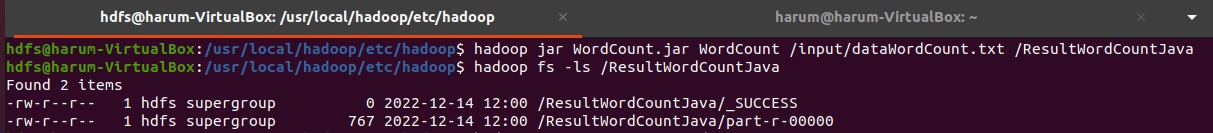
\includegraphics[width=\textwidth]{9}
\caption{Hasil Perhitungan dengan WordCount Hadoop}
\label{gam:perkuliahan-25-11}
\end{figure}

\begin{figure}[!ht]
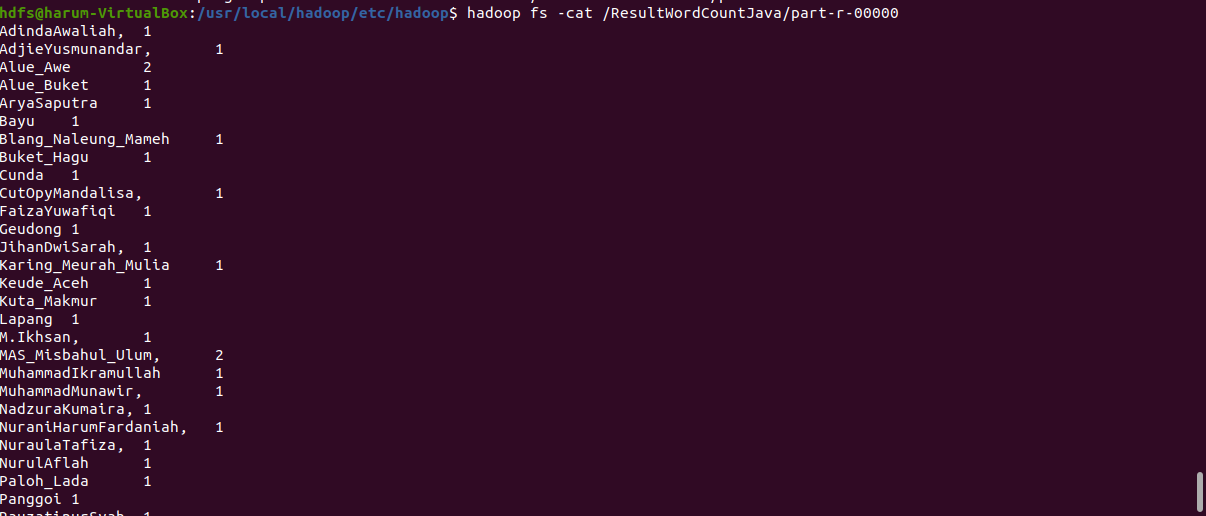
\includegraphics[width=\textwidth]{10a}
\caption{Hasil Perhitungan dengan WordCount Hadoop}
\label{gam:perkuliahan-25-11}
\end{figure}
\newpage
\begin{figure}[!ht]
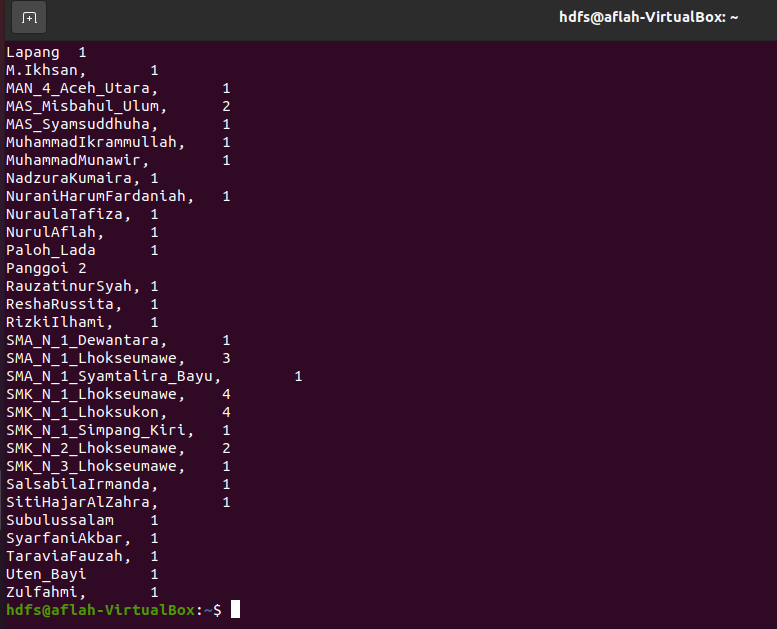
\includegraphics[width=\textwidth]{10b}
\caption{Hasil Perhitungan dengan WordCount Hadoop}
\label{gam:perkuliahan-25-11}
\end{figure}

\end{enumerate}

\newday{\textbf{9 Desember 2022}}
\begin{enumerate}
\item Kendala dan Solusi
% jelaskan kendala dan penyebab yang dialami saat mengikuti praktikum serta solusi atau langkah-langkah yang telah dilakukan

\item Kesimpulan
% berikan kesimpulan dari praktikum yang telah dikerjkan

\end{enumerate}
